% !TeX root = main.tex

\section{Experimental Evaluation}
\label{sec:experiments}
We evaluate \sorcar on two suites of benchmarks: the first suite consists of GPU programs converted to Boogie by the tool GPUVerify~\cite{DBLP:conf/oopsla/BettsCDQT12,DBLP:conf/oopsla/ChongDKKQ13}, while the second suite consists of programs that dynamically manipulate heaps and are annotated with separation logic specifications, taken from
the work in~\cite{DBLP:conf/tacas/Neider0MS018}.
The tools reported in the corresponding papers for GPUVerify~\cite{DBLP:conf/oopsla/BettsCDQT12,DBLP:conf/oopsla/ChongDKKQ13} and for proving programs against these separation logic specifications~\cite{DBLP:conf/tacas/Neider0MS018} are the best ones we know for the respective benchmark suites, and both of them use \houdini.

We compared \sorcar with the tools reported in these papers, using the same set of predicates they use.
The goals of our experiments are to measure
\begin{enumerate*}[label={(\alph*)}]
    \item the efficiency of the \sorcar algorithm in comparison with these tools that use \houdini,
    \item whether \sorcar helps to prove programs that could not be proved by the above tools (within some time bound), and vice versa, as well as
    \item how effective \sorcar is in finding smaller conjunctive invariants. % in comparison with the above tools.
\end{enumerate*}

\paragraph{Benchmarks and Compared Tools}
The first benchmark suite is taken from the 
GPUVerify tool~\cite{DBLP:conf/oopsla/BettsCDQT12,DBLP:conf/oopsla/ChongDKKQ13} and was obtained from GPU kernels written in OpenCL and CUDA.
GPUVerify converts such code automatically by a complex process involving sequentialization and compilation to the \boogie verification language.
After removing all programs that do not have loops or recursion, this benchmark suite contained $292$ programs. 

GPUVerify operates in three stages.
The first stage compiles the OpenCL or CUDA programs into Boogie programs.
The second stage uses \houdini in a custom version of \boogie to infer an inductive invariant;
in this phase, the assertions are in fact \emph{removed} as \houdini anyway is agnostic to the property being proved.
The third phase substitutes the synthesized invariants, inserts the assertions back into the \boogie program, and verifies it. 
We had to remove 3 programs from this set due to failure to compile into \boogie. 

The second benchmark consists of $63$ heap manipulating programs, originating mainly from open source projects.
These programs are written in C with specifications in \textsc{Dryad}, a dialect of separation logic that allows expressing second order properties using recursive functions and predicates.
The benchmark suit is taken from the work of Neider et al.~\cite{DBLP:conf/tacas/Neider0MS018}, which considers the problem of synthesizing invariants for sound-but-incomplete verification engines.
 
The tool developed by Neider et al.\ has the following pipeline.
First, an extension of \textsc{VCC}~\cite{vcc}, called \textsc{VCDryad}~\cite{vcdryad}, compiles the C code into a \boogie programs by unfolding recursive definitions, modeling heaplets as sets, and applying frame reasoning using a technique called natural proofs.
The tool then poses the verification problem as an invariant synthesis problem, where the incomplete verification engine, though unable to produce concrete configurations as counterexamples, still can return Horn-ICE counterexamples. 
A loop invariant is then synthesized using the \houdini engine of \boogie over a class of predicates that express complex properties of the heap (such as whether the heaplets of two data structures are disjoint, whether a list is sorted, and so on).

\begin{figure}%[H]
    \centering
    
    % !. row
    \makebox[0pt]
    {
        \subfloat[]{{\label{sf:a}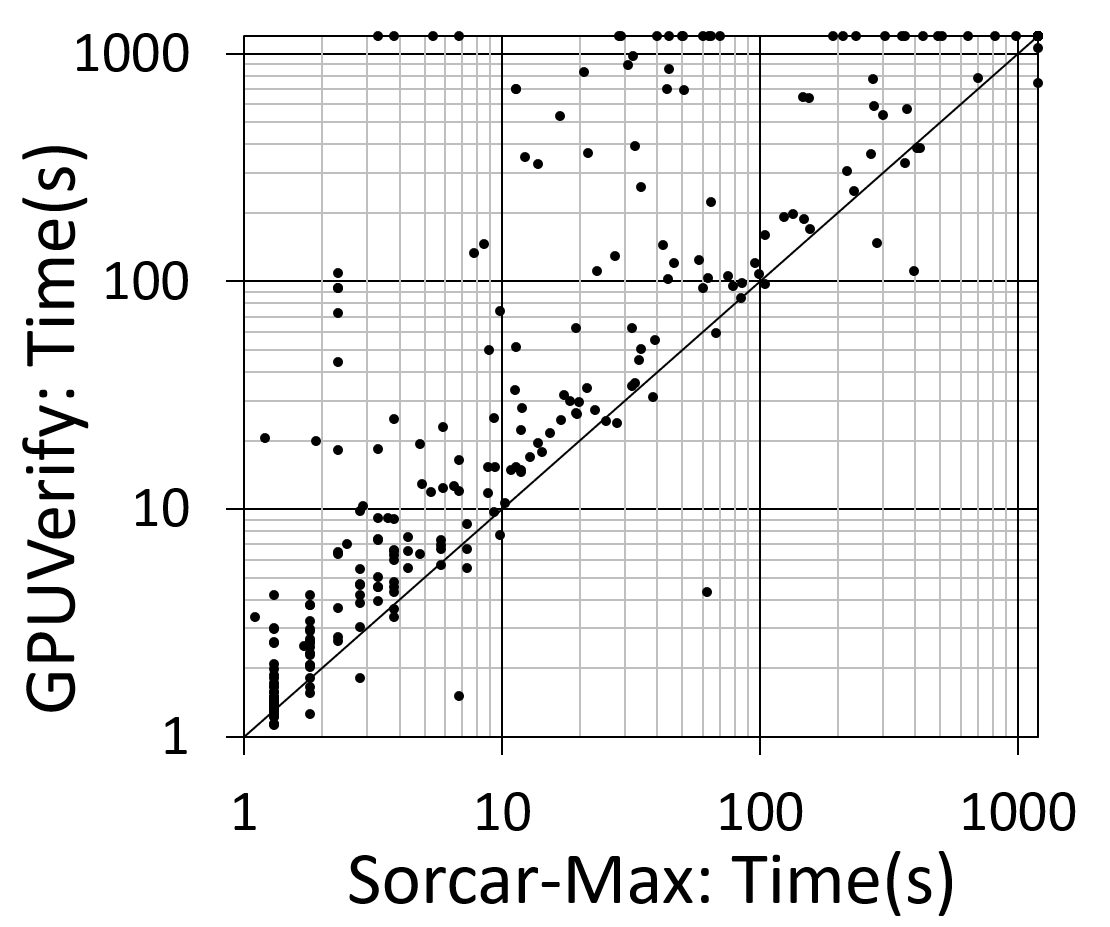
\includegraphics[width=6cm]{gpuTime.png} }}%
        \subfloat[]{{\label{sf:b}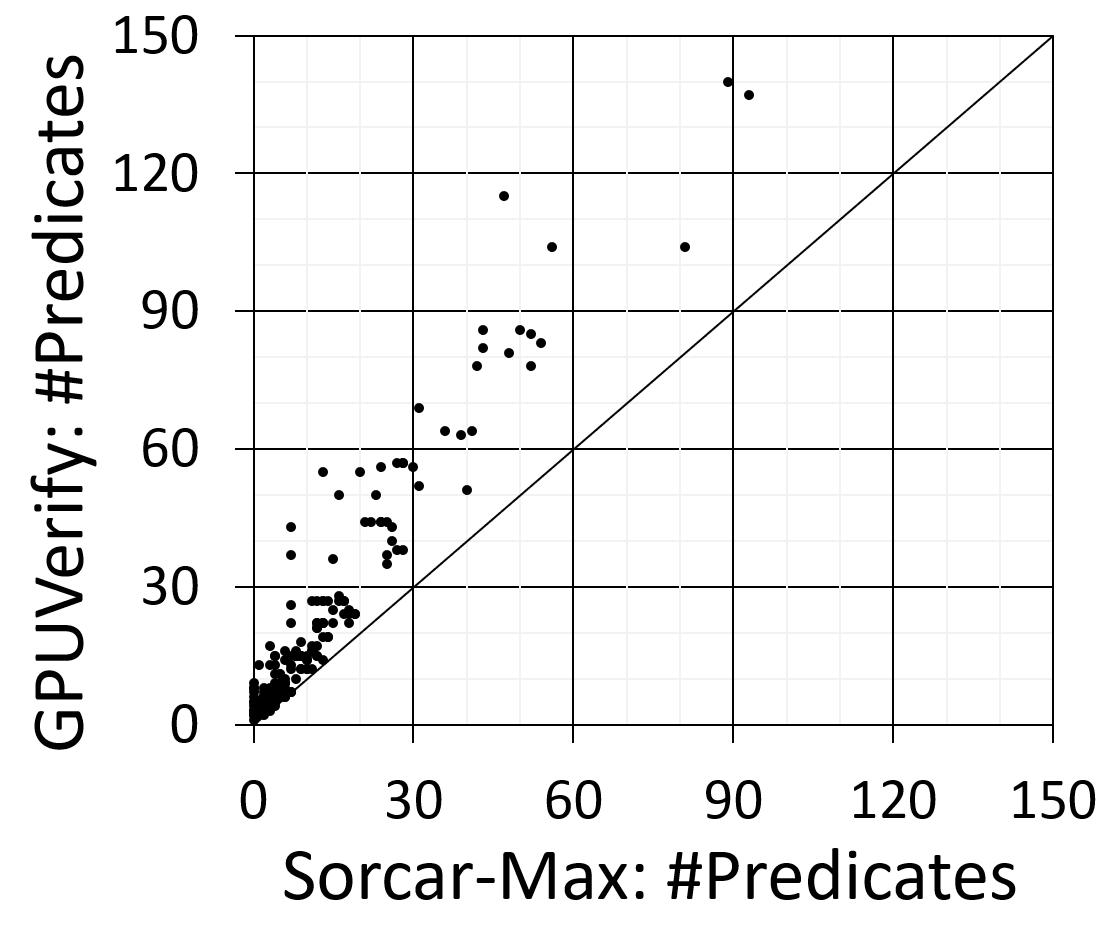
\includegraphics[width=6cm]{gpuPred.png} }}%
    }
    \\
    % 2. row
    \makebox[0pt]
    {    
        \subfloat[]{{\label{sf:c}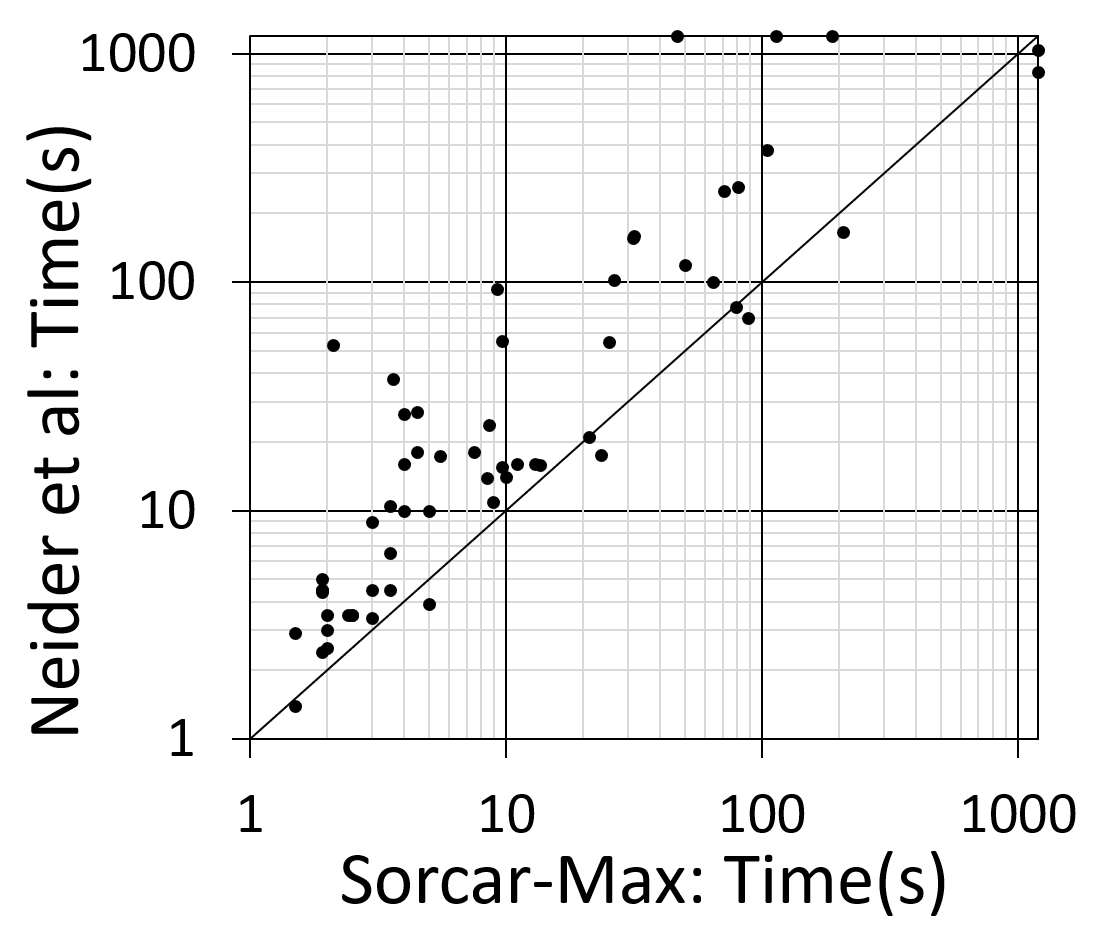
\includegraphics[width=6cm]{dryadTime.png} }}%
        \subfloat[]{{\label{sf:d}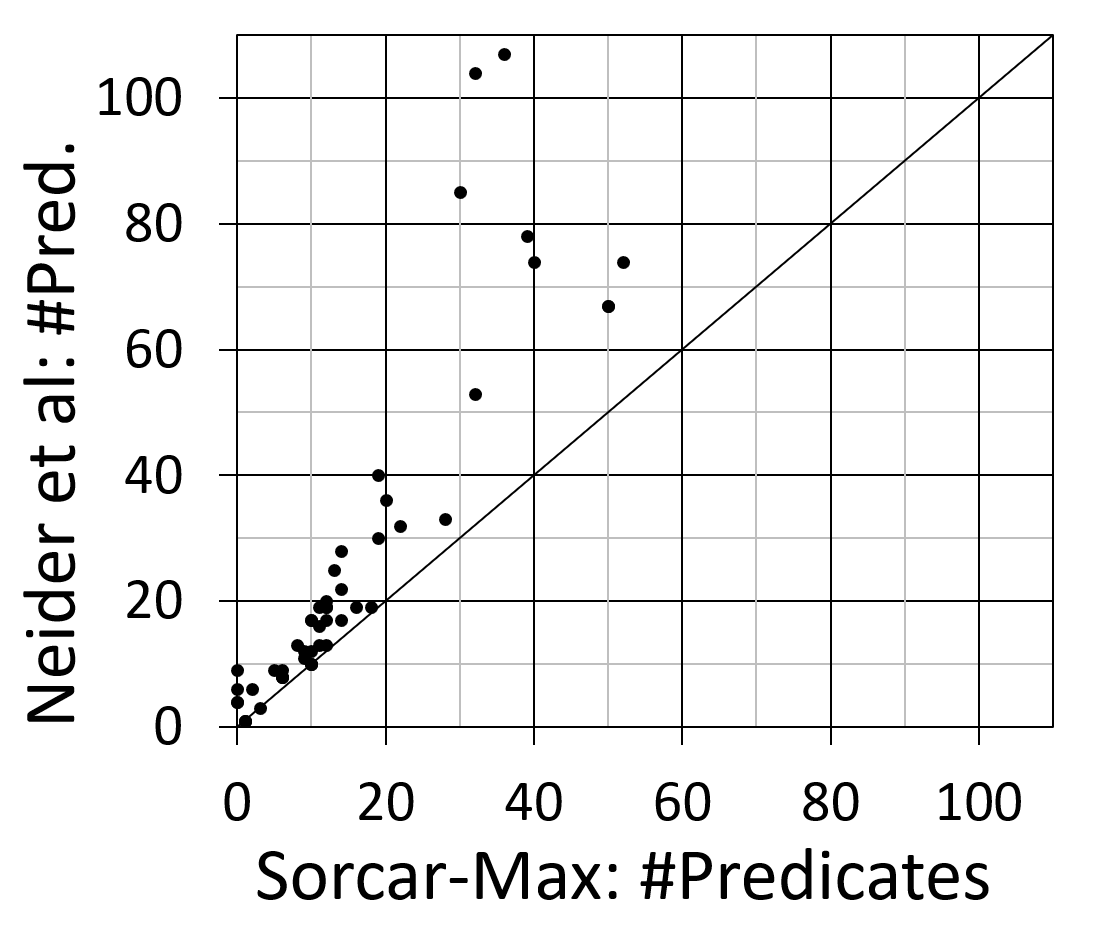
\includegraphics[width=6cm]{dryadPred.png} }}%
    }
    \\
    % 3. row
    \makebox[0pt]
    {
        \subfloat[]{{\label{sf:e}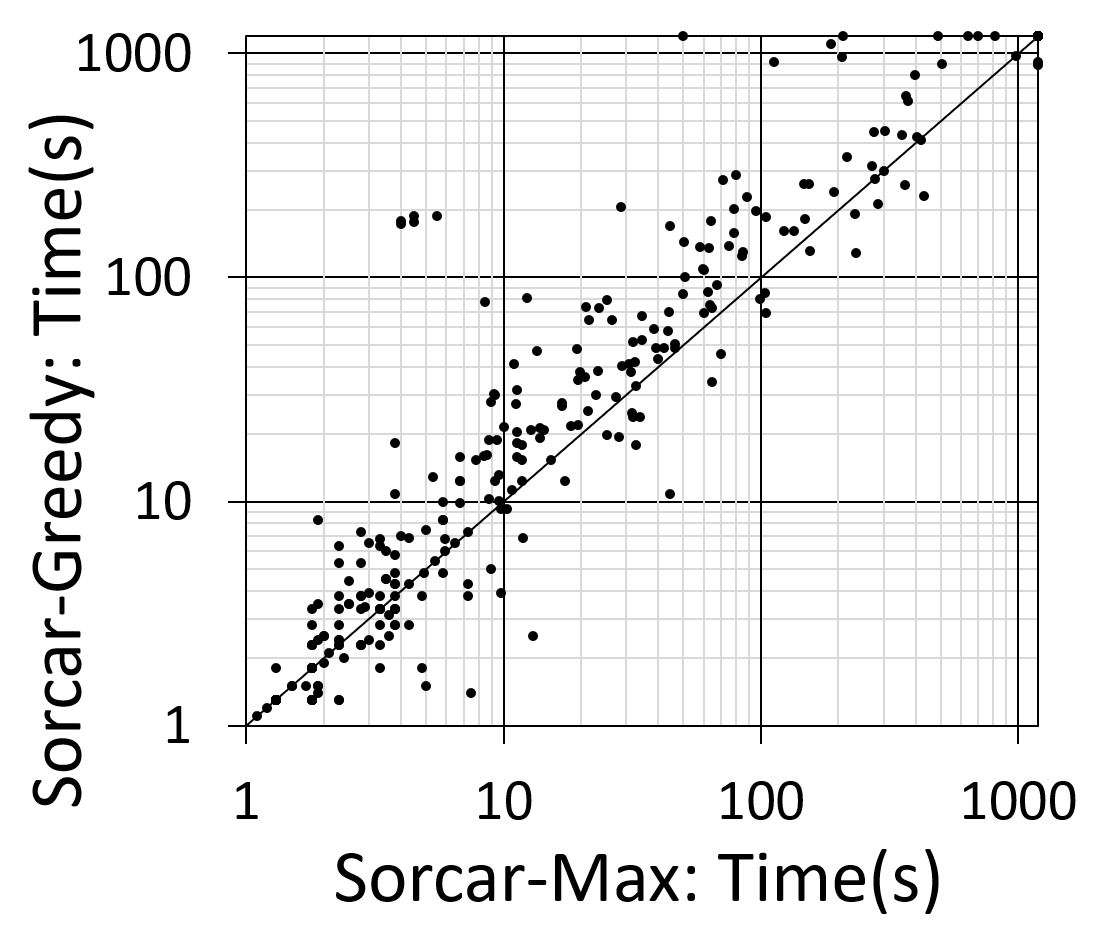
\includegraphics[width=6cm]{greedyTime.png} }}%
        \subfloat[]{{\label{sf:f}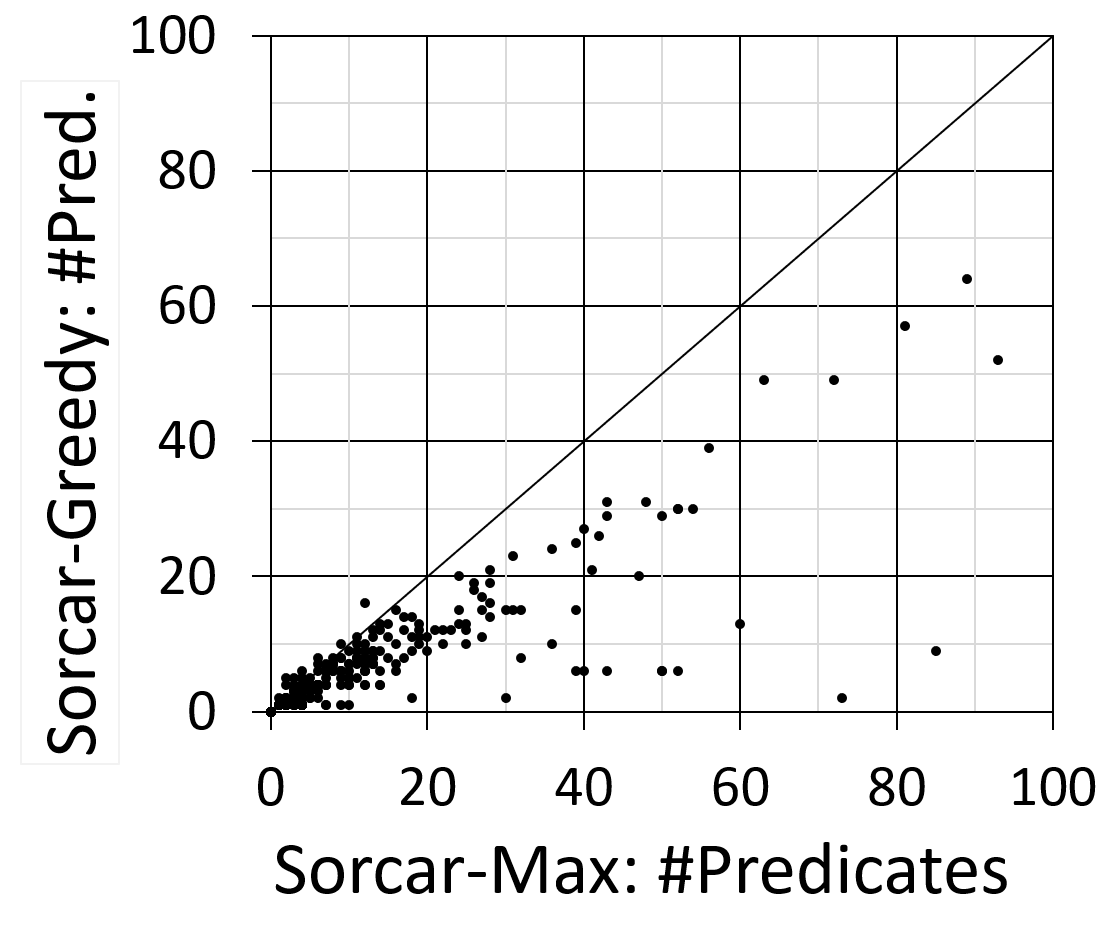
\includegraphics[width=6cm]{greedyPred.png} }}%
    }

    \caption{Comparison of time taken and number of predicates in final invariant, between the solvers \mbox{\sorcar-Max} and GPUVerify on Benchmark Suite\#1 ((a) and (b)), \mbox{\sorcar-Max} and Neider et al.'s tool on Benchmark Suite\#2 ((c) and (d)), and \mbox{\sorcar-Max} and \sorcar-Greedy over both benchmark suites (\ref{sf:e} and \ref{sf:f}).}
    \label{fig:results}
\end{figure}


%\paragraph{Implementation of Sorcar}
%\emph{Abstract Houdini} is a subframework in \boogie that allows extensions for loop invariant generation, and we implement the \sorcar algorithm (including all variants) using it.
%The algorithm is written in C+\!+ ($\sim 1800$ LOC).
%The benchmarks are transformed to the Abstract Houdini format for verification.


%---------- Evaluation ----------
\paragraph{Evaluation}
We have implemented all four variants of \sorcar in C+\!+ (approximately 1800 lines of code)\footnote{We will create an artifact and make the implementation publicly available.} and evaluated them on both benchmarks suits.
All experiments were conducted on an Intel Xeon E7-8857 v2 CPU at $3,6\,\text{GHz}$, running Debian GNU/Linux 9.5.
The timeout limit was $1200\,s$.
So as to not clutter the following presentation too much, we only report on the version of \sorcar that performed best: \textsc{Sorcar-Max} (using \RelevantPredicatesMax).
Additionally, we briefly compare \textsc{Sorcar-Max} to \textsc{Sorcar-Greedy}, which uses \RelevantPredicatesGreedy.\kern-.06em\footnote{All results can be found at \url{http://bit.ly/sorcar-evaluation}.}

Figures~\ref{sf:a} and \ref{sf:b} compare \textsc{Sorcar-Max} and GPUVerify on the first benchmark suite.
Figure~\ref{sf:a} compares the time taken by the two tools, while Figure~\ref{sf:b} compares the size of the final invariant (there is only one loop invariant in these programs).
%
As can be seen from the figures, \textsc{Sorcar-Max} compares significantly favorably in both time and size of predicates.
On programs that were able to verify, \textsc{Sorcar-Max} took on average $49\,s$ per program and synthesized invariants with an average number of $12$ conjuncts.
GPUVerify, on the other hand, took on average $96\,s$ per program and synthesized invariants with an average number of $23$ conjuncts.
Furthermore, \textsc{Sorcar-Max} was able to verify $22$ programs that GPUVerify could not verify, whereas GPUVerify verified only $2$ programs that \textsc{Sorcar-Max} could not verify. 

Figures~\ref{sf:c} and \ref{sf:d} compare \textsc{Sorcar-Max} to the tool of Neider et al.~\cite{DBLP:conf/tacas/Neider0MS018} on the second benchmark suite.
Again, \textsc{Sorcar-Max} outperformed the Houdini-based tool both in terms of time and size of invariants synthesized.
On programs that both were able to verify, \textsc{Sorcar-Max} took on average $24\,s$ per program and synthesized invariants with an average number of $25$ conjuncts.
On the other hand, Neider et al.'s tool took on average $75\,s$ per program and synthesized invariants with an average number of $41$ conjuncts.
Furthermore, \textsc{Sorcar-Max} was able to verify $3$ programs that the Neider et al.'s tool could not verify, whereas Neider et al.'s tool verified $2$ programs that \textsc{Sorcar-Max} could not verify. 

Finally, Figures~\ref{sf:e} and \ref{sf:f} compare \textsc{Sorcar-Max} and \textsc{Sorcar-Greedy}.
\textsc{Sorcar-Greedy} was slightly slower but was able to synthesizes, overall, much smaller invariants. 

%two versions of \sorcar, one that uses maximal set of relevant predicates (MAX) (Algorithm~2) and the one that uses the greedy method to find relevant predicates (GREEDY) (Algorithm~5). The greedy version of \sorcar performs a bit slower but is able to synthesizes, overall, much smaller invariants. 
%We also implemented the other variants  but we do not report on them here as the above two variants emerged as the most competitive.

%on the total time taken, and the size of the final invariant. Note that GPUVerify uses a prepossessing compilation step.  We subtract the time taken by this compilation step from the total time taken. 

%On the GPUVerify benchmarks, we evaluate the performance of the whole tool-chain, which includes a custom version of Boogie. We also set as baseline the performance of standard Boogie on the compiled Boogie programs. 
%For the Dryad benchmarks, we compare against the standard off-the-shelf Boogie.



